%%%%%%%%%%%%%%%%%%%%%%%%%%%%%%%%%%%%%%%%%%%%%%%%%%%%%%%%%%%%%%%%%%% 
%                                                                 %
%                            CHAPTER                              %
%                                                                 %
%%%%%%%%%%%%%%%%%%%%%%%%%%%%%%%%%%%%%%%%%%%%%%%%%%%%%%%%%%%%%%%%%%% 
 
\chapter{Herkenning en detectie implementatie op mobiel platform}
Dit hoofdstuk zal gaan over het implementeren van deep learning herkeningssystemen en detectiesystemen op een mobiel platform.
In dit hoofdstuk wordt er besproken welke technologi\"en er gebruikt kunnen worden om een CNN te implementeren op een mobiel platform.
Dit gaan een aantal frameworks zijn die de programeur in staat stelt om een bestaand model te implementeren op een mobiel apparaat.
Deze frameworks gaan vergeleken worden om te kijken van welk framework het best gebruik wordt gemaakt voor een bepaalde toepassing.
Er wordt ook onderzocht hoe een bestaand herkeningssystemen en detectiesystemen ge\"optimalisserd kan worden zodat dit gebruikt kan worden op een mobiel platform.
Bij het uitvoeren van een neuraal netwerk op een mobiel apparaat zal men rekening moeten houden met de volgende zaken: 
gelimiteerde rekenkracht en beschikbaar geheugen.
Ook moet er rekening gehouden worden met een beperkte batterij, want CNN's gebruiken veel bandbreedte en voeren veel berekeningen uit wat meer energie verbruikt.
Dus er zal onderzocht moeten worden welke methodes men kan gebruiken om het geheugen van het model, het aantal bewerkingen en het energieverbruik te kunnen verbeteren.
%refereren

\section{Van object detectie model naar een mobiele Implementatie}
Om machine learning modelen te ontwerpen en te trainen kan er gebruik gemaakt worden van frameworks.
Deze frameworks geven de programeur een set van tools die hun in staat stelt om op een overzichtelijke en flexibele manier machine learning modellen te ontwerpen en trainen.
In deze paragraaf worden enkele van de meest gebruikte frameworks besproken.
Dit zijn enkele van de meest gebruikte frameworks, maar zeker niet allemaal.

\section{Frameworks}
TensorFlow en PyTorch zijn de 2 voornaamste frameworks die gebruikt worden om neurale netwerken te ontwerpen en trainen.
Veel van de tools en bibliotheken die gebruikt worden om herkeningssystemen en detectiesystemen te ontwerpen worden bovenop deze frameworks gebruikt.

\subsection{TensorFlow}
TensorFlow (\cite{abadi_tensorflow_2016}) is ontworpen door Google en is een open source library voor machine learning implementaties.
TensorFlow focust op het trainen en het deployen van neurale netwerken.
Ook ondersteund TensorFlow meerdere programeer talen zoals: Python, Java en C.
Door de introductie van de Keras API is TensorFlow meer gebruiksvriendelijk geworden.
Keras is een framework dat bovenop TensorFlow gebruikt kan worden, waarmee machine learning modellen kunnen ontworpen worden op een overzichtelijke manier.
%Keras refereren
Zo heeft TensorFlow een gebruiksvriendelijk API voor eenvoudige projecten en meer uitgebreide tools voor complexe projecten.
%TensorFlow kan  dynamisch zijn grafieken wanneer variabelen worden gedeclareerd.
Door gebruik te maken van TensorBoard kan data op een flexibele manier gevisualiseerd worden tijdens runtime. 
TensorFlow biedt ook goede ondersteuning op gebied van deployment van een productie model.
Nog een voordeel van TensorFlow is dat het een grootte community achter zich heeft, omdat dit een veel gebruikt framework is.
%extra sectie voor Keras

\subsection{PyTorch}
PyTorch (\cite{li_PyTorch_2020}) is ontworpen door facebook en wordt zoals TensorFlow ook gebruikt voor machine learning implementaties.
Dit is een python gebaseerd framework dat focust op flexibiliteit, maar deze extra flexibiliteit zorgt voor meer lijnen code.
Door zijn flexibiliteit is het gemakkelijk om nieuwe functionaliteiten toe te voegen door bestaande code aan te passen of nieuwe code toe te voegen.
PyTorch maakt gebruik van externe tools zoals TensorBoard om data te visualiseren.
Dit framework wordt gebruikt om een machine learning model te ontwerpen en trainen.
Het model dat is ontworpen kan vervolgens gebruikt worden gebruikt om een applicatie te ontwerpen.
%Vermits PyTorch voornamelijk focust op het ontwerpen van netwerken zal dit in deze masterproef minder van toepassing zijn.

%vergelijking tf en PyTorch
PyTorch wordt voornamelijk gebruikt om te experimenteren met neurale netwerken.
Bedrijven en onderzoekers gebruiken dit framework vooral om een CNN experimenteel op te bouwen en te trainen.
TensorFlow wordt voornamelijk gebruikt om het model effectief in gebruik te nemen.
%De TensorFlow Lite conversie geeft meer zekerheid t.o.v. de PyToch Mobile conversie vermits deze nog in zijn Beta fase zit.

\section{Object detectie bibliotheken}
Er zijn heel wat bibliotheken die de programeur kan importeren.
Deze bibliotheken geven de programeur extra tools en hulpmiddelen om een detectiesysteem te ontwerpen en te trainen.

\subsection{MMDetection}
MMDetection maakt deel uit van OpenMMLab en is een open source object detectie toolbox gebaseerd op PyTorch.
De toolbox bevat gewichten van meer dan 200 voorgetrainde modellen.
Via modulair ontwerp kan het detectie framework opgesplitst worden in verschillende componenten.
Met de verschillende componenten kan een eigen detectie model worden gemaakt door de verschillende componenten te combineren.
MMDetection ondersteund ook 48 verschillende detectie methodes zoals: YOLO, Faster R-CNN, etc.
Al de bounding box en masker operaties worden uitgevoerd op GPU's dit geeft MMDetectie een grootte trainingssnelheid.
MMDetection biedt geen ondersteuning om een bestaand model te optimaliseren naar een model voor mobiele toepassingen.
Dus dit model zal geconverteerd moeten worden naar een framework waarbij het optimaliseren naar een mobiel model wel mogelijk is.
%suports COCO en VOC style datasets

\subsection{Detectron2}
Detectron2 is een bibliotheek van Facebook die segmentatie en detectie algoritmes ondersteunt.
Zoals MMDetection werkt Detectron2 bovenop Pytorch en kan het netwerk getraind worden op 1 of meerdere GPU's.
Via Modular, extensible design kan Detectron2 specifieke modules toevoegen aan bijna elk deel van een object detectiesysteem.
Detectron2 bevat meer dan 80 voorgetrainde modellen waarop de programeur verder kan bouwen.
Voor object detectie ondersteund Detectron2 6 verschillende standaard modellen.

\subsection{Darkflow}

\subsection{ImageAI}
ImageAI is makelijk te gebruiken Python bibliotheek die de programeur in staat stelt om State-of-the-art AI feautres te implementeren.
ImageAI ondersteund object detectie door gebruik te maken van RetinaNet, YOLOv3 en TinyYOLOv3 getraind met de COCO dataset.
Deze bibliotheek werkt sinds juni 2021 bovenop PyTorch, hiervoor werkte ImageAI bovenop TensorFlow.
Ook deze bibliotheek geeft de programeur de mogelijkheid om nieuwe modellen te trainen om specifieke objecten te detecteren.


\section{Frameworks voor mobiele implementatie}
Er zijn een aantal frameworks die de programeur de mogelijkheid geven om een model te optilmaliseren voor een mobiel platform.
Er zal voornamelijk gefocust worden op Android implementaties.
Niet elke framework voor mobiele implementatie optimaliseert het model op dezelfde manier.
Zo zullen sommige modellen na het optilmaliseren in een bepaald framework een kleinere bestands grootte hebben dan bij andere frameworks.
Of sommige frameworks zullen beter optimaliseren op gebied van latency of accuraatheid dan andere frameworks.

\subsection{CoreML}
Core ML is het Apple framework om machine learning tools te integreren in een applicatie.
Dit kan een model zijn van Create ML het machine learning framework van Apple zelf.
Maar Core ML biedt ondersteuning om modellen te converteren van TensorFlow, PyTorch en ONNX naar Core ML.
Uiteraard is dit framework enkel van toepassing voor Apple, en in deze masterproef wordt er vooral gefocust op een Android implementatie.

\subsection{Mobile AI Compute Engine (MACE)}
Het MACE framework is ontworpen door Xaomi en dient specifiek voor mobiele toepassingen van neurale netwerken op Android, IOS, Linux en Windows.
MACE biedt ondersteuning voor verschillende frameworks zoals: TensorFlow, Caffe en ONNX.
Het model kan ge\"implementeerd worden op Android, IOS en Linux.
Het MACE framework bespaart geheugen door de core library zo klein mogelijk te maken door het aantal externe dependencies te minimaliseren.
Het Winograd algoritme ... wordt gebruikt om convolutie bewerkingen te versnellen en verbeterd op deze manier de latency van het CNN model.

\subsection{TensorFlow Lite}
\begin{figure}[!ht]
    \centering
 	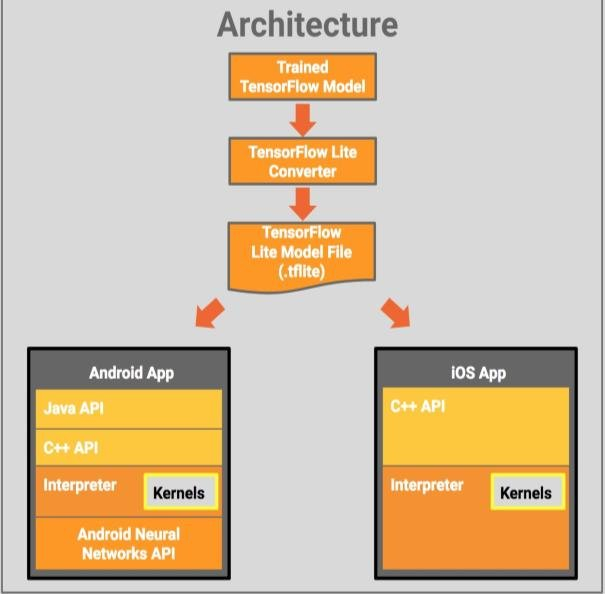
\includegraphics[width=0.5\linewidth]{fig/TFLite.jpg}
 	\caption{Implementatie flow van een getraind TensorFlow model naar de applicatie}
 	\label{fig:tflite}
\end{figure}

%anders formuleren
TensorFlow Lite is het antwoord van TensorFlow om CNN modellen te optimaliseren voor mobiel gebruik (figuur: \ref{fig:tflite}).
TensorFlow Lite zorgt ervoor dat het model een lage latency heeft en een kleine binaire grootte.
Het converteren kan makkelijk worden uitgevoerd via de volgende lijnen code in Python.

\begin{lstlisting}[language=Python, caption=Converteren van TensorFlow naar een TensorFlow Lite model]
import tensorflow as tf

converter = tf.lite.TFLiteConverter.from_saved_model(saved_model_dir)
tflite_model = converter.convert()
\end{lstlisting}	

Het TensorFlow Lite framework geeft ook de mogelijkheid om verdere optimalisaties zoals pruning en quantisatie uit te voeren na het converteren.
Het TensorFlow Lite model is ook compatibel met android en IOS.
Bij Android kan TensorFlow gebruik maken van de Neural Network API (NNAPI) ... die beschikbaar is vanaf Android 8.1.
Deze API kan gebruikt worden om netwerk modellen te versnellen met de GPU, DSP en NPU.

\subsection{PyTorch Mobile}
\begin{figure}[!ht]
    \centering
 	\includegraphics[width=0.5\linewidth]{fig/PyTorch-mobile.png}
 	\caption{Implementatie flow van een getraind PyTorch model naar de applicatie met code}
 	\label{fig:pt_mobile}
\end{figure}

PyTorch biedt zoals TensorFlow ook de mogelijk om het model te optimaliseren naar PyTorch Mobile.
In figuur: \ref{fig:pt_mobile} is te zien welke lijnen code er moeten worden uitgevoerd om een PyTorch model te converteren naar een PyTorch mobile model.
PyTorch mobile zit nog in zijn beta fase, dus hierbij kunnen er onverwachte complicaties optreden.
Een ander framework is Caffe2 dit framework focust ook op mobiele implementaties, maar het framework is ondertussen ge\"intrigeerd met PyTorch.
Ook is het PyTorch framework compatibel met android en IOS.
%meer over caffe


%TVM en qualcom

In de paper geschreven door \cite{luo_comparison_2020} wordt PyTorch Mobile vergeleken met Tenserfolow Lite voor verschillende netwerk architecturen en een model getraind met dezelfde data.
Voor alle netwerk architecturen in deze paper geeft de optimalisatie naar TensorFlow Lite de kleinste bestand grootte van het model. 
Uit deze paper is ook af te leiden dat de optimalisatie naar een mobiel model niet alleen afhankelijk is van het framework maar ook van de netwerk architectuur.
Zo geeft TensorFlow Lite volgens \cite{luo_comparison_2020} betere latency resultaten voor de zwaardere netwerken (ResNet50, InceptionV3, DenseNet121) dan PyTorch Mobile.
Maar PyTorch Mobile heeft op zijn beurt wel een betere latency voor SqueezeNet en MobileNetV2.
Dus uit deze paper kunnen we afleiden dat TensorFlow Lite het beste de bestands grootte verkleint, maar dat de netwerk architectuur ook een rol speelt.

\cite{febvay_low-level_2020} vergelijkt TensorFlow Lite met MACE voor verschillende neurale netwerken (SqueezeNet, MobileNetV1/V2).
Hierbij geeft TensorFlow Lite het beste resultaat, TensorFlow Lite gaf een Top-1 resultaat van 69,19\% en MACE gaf een top-1 resultaat van 66.84\% bij MobileNetV1.
Ook voor de latency gaf TensorFlow Lite in de meeste gevallen de beste resultaten buiten bij het gebruik van 4 of 6 CPU cores, dan gaf MACE betere resultaten.  

\section{Converteren naar framework voor mobiele implementatie}
Het doel van deze masterproef is om een bestaand netwerk op een mobiel platform te krijgen.
Dus zullen de object detectoren die ontworpen zijn met bovenstaande tools (Detectron2, MMDetection, ImagAI en Darkflow), geconverteerd moeten worden naar een framework voor mobiele implementatie.
Object detectoren zijn complexe systemen waarbij het converteren naar een ander framework complex of zelfs niet mogelijk zal worden.
In deze paragraaf zal per objectdetector bibliotheek gekeken worden wat de mogelijkheden zijn om van een detector model naar een mobiele implementatie te gaan.
De eerste stap zal zijn om te kijken welke mogelijkheden er zijn zonder te converteren naar een ander framework.
Een tweede stap is via Open Neural Network Exchange (ONNX) het huidige detectie model converteren naar een andere framework.
Een derde stap is verder zoeken naar een alternatief als de eerste twee methodes niet lukken.

%ONNX
\subsection{ONNX}
\cite{onnx_onnx_2017} biedt de mogelijkheid om verschillende tools/frameworks samen te laten werken.
Hierbij wordt een bestaand model geconverteerd naar een ONNX model, en dit model kan op zijn beurt geconverteerd worden naar het gewilde framework.
ONNX ondersteund niet elk machine learning framework, maar toch wel de meest bekende.
Het ONNX framework biedt zelf ook de mogelijkheid om een model te deployen en te optimaliseren voor mobiel gebruik.
ONNX dient goed als overkoepelend framework dat er voor zorgt dat verschillende frameworks compatibel zijn met elkaar.
Volgens de website zijn er 23 frameworks die naar het ONNX framework geconverteerd kunnen worden en een CNN kunnen ontwerpen en trainen. 
Om dan geconverteerd te worden naar een framework dat het model kan omzetten naar een mobile versie.
Een ander manieren om een model te gebruiken over verschillende frameworks in plaats van ONNX hangt af van de compatibiliteit tussen frameworks.
Bepaalde frameworks zullen zelf een methode hebben om modellen van andere frameworks in te laden.

\subsection{Van MMDetection naar detectie model voor mobile implementatie}
%MMDetection
Voor het testen van MMDetection nemen we de Kitty dataset ... waarmee we een detector trainen via transfer learning, hiervoor gebruiken we de Mask-rcnn detector.
Vermits MMDetection bovenop PyTorch werkt gaan we eerst proberen om met PyTorch Mobile te werken, dit gaat via de volgende lijnen code.

\begin{lstlisting}[language=Python, caption=Converteren van MMDetection naar een PyTorch Mobile]
import torch
import torchvision
from torch.utils.mobile_optimizer import optimize_for_mobile

model.eval()
example = torch.rand(1, 3, 224, 224)
traced_script_module = torch.jit.trace(model, example)
traced_script_module_optimized = optimize_for_mobile(traced_script_module)
traced_script_module_optimized._save_for_lite_interpreter("model.ptl")
\end{lstlisting}

Voordat het model kan geoptimaliseerd worden moet het python afhankelijk model worden omgezet in TorchScript. 
Deze TorchScript module kan dan verder geoptimaliseerd worden voor mobiel gebruik.
Het omzetten naar de scriptmodule geeft een TypeError fout waardoor het optimaliseren voor mobiel niet lukt.

Een andere manier om naar een mobiele implementatie te gaan is door het model eerst om te zetten naar het .onnx formaat.
MMDetection ondersteund de conversie naar ONNX, maar dit zit nog in zijn experimentele fase.
In de documentatie van MMDetection kan er een lijst gevonden worden met detectiemodellen die ondersteuning hebben voor het exporteren naar ONNX ... .
Ook heeft ONNX 'opsets' met daarin de operaties die ONNX ondersteund, niet elk framework past dezelfde opset versie toe wat later voor problemen kan zorgen.
Elke bibliotheek/framework moet dezelfde 'opset' implementeren anders zullen er operaties zijn die niet compatibel zijn met het gewilde framework voor mobiele implementatie.
Via de volgende lijn code is het mogelijk om het MMDetection model om te zetten naar een ONNX model.

\begin{lstlisting}[language=Python, caption=Converteren van MMDetection naar een onnx bestand]
!python ./tools/deployment/pytorch2onnx.py <config_file> <checkpiont_file> 
	--output-file <output file>
\end{lstlisting}

pytorch2onnx.py is het MMDetection script om een model te converteren naar ONNX formaat.
De config file is het bestand dat het neuraal netwerk beschrijft.
En de checkpoint file is een file die tijdens het trainen wordt aangemaakt als checkpoint.
Het finale model is vaak terug te vinden als latest.pth, dit is het laatste checkpoint dat na het trainen wordt aangemaakt.
Op het einde van deze lijn code is het mogelijk om nog extra opties toe te voegen die in de MMDetection documentatie ... terug te vinden zijn.
Bovenstaande lijn code converteert het MMDetection model succesvol naar een ONNX model.
Wel moet er bij vermeld worden dat dit MMDetection model een \'e\'envoudig model is waarbij geen speciale aanpassingen zijn gedaan.
Dus bij complexere modellen zou het resultaat anders kunnen zijn.

Het gegenereerde .onnx model is vervolgens geconverteerd naar een TensorFlow Lite model via de volgende lijnen code.

\begin{lstlisting}[language=Python, caption=Converteren van ONNX bestand naar een TensorFlow Lite model]
import tensorflow as tf
import onnx
from onnx_tf.backend import prepare
	
#ONNX model inladen 
onnx_model = onnx.load("model.onnx")  # inladen onnx model
output = prepare(onnx_model)
output.export_graph('tf_model.pb') # model exporteren naar TensorFlow model

#Ingeladen model omzetten naar TensorFlow Lite model
converter = tf.lite.TFLiteConverter.from_saved_model('tf_model.pb')
converter.target_spec.supported_ops = [
	tf.lite.OpsSet.TFLITE_BUILTINS, # enable TensorFlow Lite ops.
	tf.lite.OpsSet.SELECT_TF_OPS # enable TensorFlow ops.
]
tflite_model = converter.convert() # converteer model
\end{lstlisting}

Eerst moet het ONNX model ingeladen worden als een standaard TensorFlow model.
Vervolgens moest bij het converteren naar een TensorFlow Lite model eerst vermeld worden welke opsets er ondersteund moeten worden.
Het effectief converteren naar een TensorFlow Lite model duurt een hele tijd .... .

Om een model te converteren naar CoreML zijn er 3 mogelijkheden.
Eerst is rechtstreeks converteren vanuit PyTorch, daarvoor moeten we eerst ons model omzetten in een torchscript.
Maar dan stoot men op hetzelfde probleem als bij de PyTorch Mobile implementatie, waarbij het omzetten naar torchscript een TypeError geeft.
De tweede manier is via ONNX maar dat raad Apple af omdat dit in de volgende versie van CoreML niet meer ondersteund wordt, CoreML biedt ook maar ondersteuning tot en met opset versie 10.
Vanuit ONNX converteren gaat via de volgende lijnen code, maar vermits dit in later versies niet meer ondersteund wordt is deze methode niet uitgetest.

\begin{lstlisting}[language=Python, caption=Converteren van ONNX bestand naar een CoreML model]
import coremltools as ct

model  = ct.converters.onnx.convert(model='my_model.onnx')
\end{lstlisting}

De derde manier is rechtstreeks via TensorFlow convert, maar dit is een vrij omslachtige manier omdat we dan de volgende converties moeten maken MMDetection -> ONNX -> TensorFlow -> CoreML.
%heeft geen keras model wanneer het van tf komt.

%onnxruntime

%mace

\subsection{Van Detectron2 naar mobile implementatie}
%Detectron2

\subsection{Van ImageAI naar mobile implementatie}
%ImageAI

\subsection{Van DarkFlow naar mobile implementatie}
%DarkFlow


\section{Van een object herkening model naar een mobiele implementatie}

\section{Implementatie op mobiele platformen}
%meer tijd spenderen aan het vergelijken tussen verschillende frameworks, en hoe een bestaand model op een mobiel apparaat
%te krijgen
Uit paragraaf 3.1 kan er afgeleidt worden dat sommige frameworks ondersteuning bieden voor het optimaliseren van het machine learning model naar een lichtere versie.
Dus het bestaande CNN model zou naar \'e\'en van deze frameworks geconverteerd moeten worden zodat er gebruik gemaakt kan worden van de mobiele optimalisatie die dat framework ondersteund.
Niet elk framework zal even compatibel zijn met het bestaande model, er zal dus gekeken moeten worden tussen welke frameworks een conversie mogelijk is.
Ook zal niet elk framework de optimalisatie voor mobiele platformen op dezelfde manier toepassen.
Dus het converteren van het standaard model naar het mobiele model zal voor elk framework een ander resultaat geven.
In deze paragraaf zal er besproken worden welke frameworks er compatibel zijn met elkaar en welke frameworks het beste optimaliseren voor een mobile implementatie.

We hebben al gezien dat voor het converteren van een model niet veel lijnen code nodig zijn. 
Maar dit is enkel het geval als het model in het zelfde framework is ontworpen.
Als het model in een ander framework is ontworpen en getraind is de eerste stap van het process om het CNN model naar het gewilde framework te converteren.


\section{Optimalisaties van neurale netwerken voor snelheid en bestandgrootte}
In deze paragraaf wordt er onderzocht welke optimalisaties er kunnen worden toegepast om de accuraatheid, snelheid en gebruikt geheugen te verbeteren.
Maar het optimaliseren van een bepaalde factor zal vaak negatieve gevolgen hebben voor een andere factor, dit zal meestal de accuraatheid zijn.
Dus er zal een goede belans gevonden moeten worden tussen de optimalisatie en de negatieve gevolgen op de andere factoren.

%\subsection{Deep compression}
%De Deep compression methode voorgesteld door \cite{han_deep_2016} gebruikt 3 technieken om een model te verkleinen zodat het bruikbaar is op een mobiel apparaat.
%De 3 technieken zijn pruning, trained quantization en Huffman coding.
%Het doel van deze 3 technieken is om de opslag vereisten te verkleinen, met zo weinig mogelijk effect op de accuraatheid.

\subsection{Pruning}
Pruning is de eerste stap van de Deep comression methode voorgesteld door \cite{han_deep_2016}.
Bij het trainen van een CNN hebben bepaalde gewichten een grotere invloed op het resultaat.
Andere gewichten hebben weinig tot geen invloed op het resultaat.
Maar alle gewichten worden steeds berekend ongeacht hun invloed op het resultaat.
Bij pruning worden de gewichten met een kleine invloed op het resultaat verwijderd dit is weergegeven op figuur \ref{fig:pruning}. 
Waardoor er geen berekeningen meer moeten uitgevoerd worden voor de verwijderde gewichten.
Deze parameters moeten dan ook niet meer worden bijgehouden waardoor het CNN model minder geheugen in beslag neemt.
Eerst wordt het CNN op een normale manier getraind zonder pruning.
Vervolgens worden al de kleine gewichten onder een bepaalde treshold verwijderd.
volgens \cite{han_deep_2016} wordt voor VGG-16 het aantal parameters met factor 13 verminderd, voor AlexNet met een factor 9.
Deze methode heeft zeer weinig tot geen effect op de accuraatheid.
%connectie pruning, neuron pruning

\begin{figure}[!ht]
	\centering
	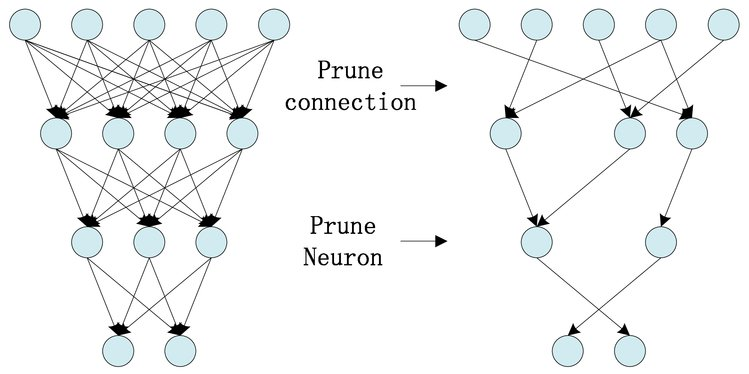
\includegraphics[width=0.65\linewidth]{fig/pruning.jpg}
	\caption{CNN voor en na pruning}
	\label{fig:pruning}
\end{figure}

\subsection{Parameter quantisatie}
Het quantiseren en delen van gewichten is een tweede methode voorgesteld door \cite{han_deep_2016}.
Een CNN bestaat uit miljoenen gewichten, en de waarde van elke van deze gewichten moeten op het systeem worden opgeslagen.
De default representatie van een waarde wordt opgeslagen als een floating point nummer wat 4 bytes in beslag neemt.
Dus voor miljoenen parameters hebben de gewichten veel schijfruimte nodig.
Een mogelijke oplossing hiervoor is quantiseren van gewichten, waarbij de getal representatie van de gewichten wordt verandert naar fixed point.
Hierbij worden de waarden van gewichten beperkt tot een set van beschikbare waardes.
Waarbij de waardes \"e\"enmalig worden opgeslagen en al de gewichten refereren naar een waarde van de vaste set met waardes.
Hoe kleiner de set met waardes is hoe minder geheugen er in beslag wordt genomen, maar een kleinere set van waardes zorgt ook voor een mindere accuratie.
Dus de grootte van de set moet goed worden gekozen zodat er niet te veel geheugen wordt gebruikt met een accepteerbare daling in accuratie.
\cite{han_deep_2016} past vervolgens Huffman encoding toe die een compressie uitvoert op de gekwantiseerde parameters.
%hashed net gebruikt hashes

\subsection{Convolutionele filter compressie}
een andere methode voorgesteld is Compressed Convolutional Filters.
Hierbij wordt de grootte van de kernel verkleind om het aantal parameters en rekenwerk te verminderen.
Maar door de kernels te verkleinen daalt de accuraatheid van het CNN.
%paper zoeken met weer uitleg

\subsection{Matrix factorisatie}
Hierbij worden grootte en complexe matrices opgesplitst in verschillende kleinere en simpelere matrices.

%\subsection{Vermijd fully connected lagen}
%Fully connected lagen zijn een basis component van neurale netwerken.
%Maar fully connected lagen genereren veel parameters, dus gebruiken ook veel geheugen.
%Ook voeren fully connected lagen veel berekening uit waardoor zij ook een vertragende factor zijn.
%Dus voor mobiele implementaties is het beter om geen of weinig fully connected lagen te gebruiken.

%\subsection{Wijzigen van de Kernel}
%Door met meer kernels te werken kan men meer informatie uit de data halen, maar dan worden er ook meer feature mappen gegenereerd.
%Deze feature mappen beschikken over veel informatie maar nemen meer geheugen in beslag.
%Een groter aantal feature mappen is meer data dus ook meer berekeningen en meer berekeningen maakt het systeem trager.
%Dus door het aantal kernels te verminderen worden er ook minder feature mappen gegenereerd.
%Dit zorgt voor een snelheids winst en meer vrij geheugen, maar er is dan wel een verlies aan informatie.

%De grootte van de kernel kan ook woorden aangepast zo kan men i.p.v. een 3x3 kernel met een 2x2 kernel werken.
%Door de kernelgrootte te verkleinen moeten er minder berekeningen worden uitgevoerd wat zorgt voor een snelheidswinst en meer vrij geheugen.
%Maar de door de kernelgrootte te verkleinen is er terug een verlies aan informatie.

%stride

%\subsection{Pooling laag optimalisatie}
%De pooling laag zorgt voor een vermindering in de dimensie van de feature map.
%deze vermindering van dimensie zorgt ervoor dat er minder parameters zijn, maar minder parameters betekent ook verlies aan informatie.
%Dus door wijzigingen aan te brengen aan de pooling laag kan de hoeveelheid data en rekenwerk verbeterd worden.

%De pooling laag kan naar voor worden geschoven in het CNN waardoor de dimensie van de feature map sneller kleiner wordt.
%Dit heeft als gevolg dat er met minder parameters verdergegaan moet worden, waardoor het model sneller wordt.
%Maar dit zorgt er ook voor dat bepaalde informatie sneller verloren gaat wat zorgt voor een lagere accuratie.
%Een andere vorm van pooling optimalisatie is gewoonweg meer pooling lagen toevoegen waardoor de dimensie van de feature mappen vaker verkleint wordt.
%Maar dit heeft ook een negatieve invloed op de accuraatheid.
%kernel vergroten

% \section{CNN architecturen voor mobiele platformen}
% Dit deel gaat over CNN architecturen die specifiek ontworpen zijn voor mobiele en embedded toestellen.
% Deze netwerk architecturen streven naar zo weinig mogelijk parameters en een zo snel mogelijke uitvoering zonder een te groot effect op de accuraatheid te hebben.
% Het overlopen van deze netwerken voor de masterproef is iets minder relevant vermits we een reeds getraind CNN willen optimaliseren.
% Dus dat netwerk is reeds getraind, maar er kan wel gekeken worden welke technieken deze architecturen gebruiken zodat het model gebruikt kan worden op een mobiel platform.

% \subsection{MobileNet}
% MobileNet is voornamelijk opgebouwd uit diepe afzonderlijke convoluties(depthwise separable convolution), om het aantal berekeningen te verminderen.
% Deze convoluties bestaan uit een depthwise convolutie, waarbij \'e\'en filter over elk input kanaal gaat waardoor er afzonderlijke feature maps onstaan.
% Vervolgens gebeurt er een pointwise convolutie die met een 1x1 convolutie de outputs samenvoegt.
% Deze manier van werken zorgt voor een grootte vermindering in het aantal parameters met een klein effect op de accuraatheid.
% VGG-16 heeft 138 miljoen parameters en een accuraatheid van 71.5\%, MobileNet heeft 4.2 miljoen parameters met een accuraatheid van 70.6\%.
% Ondertussen is er al een MobileNetV2 ... en ook een MobileNetV3 ... .

% \subsection{EfficientNet}


% \subsection{TinyYOLO}
